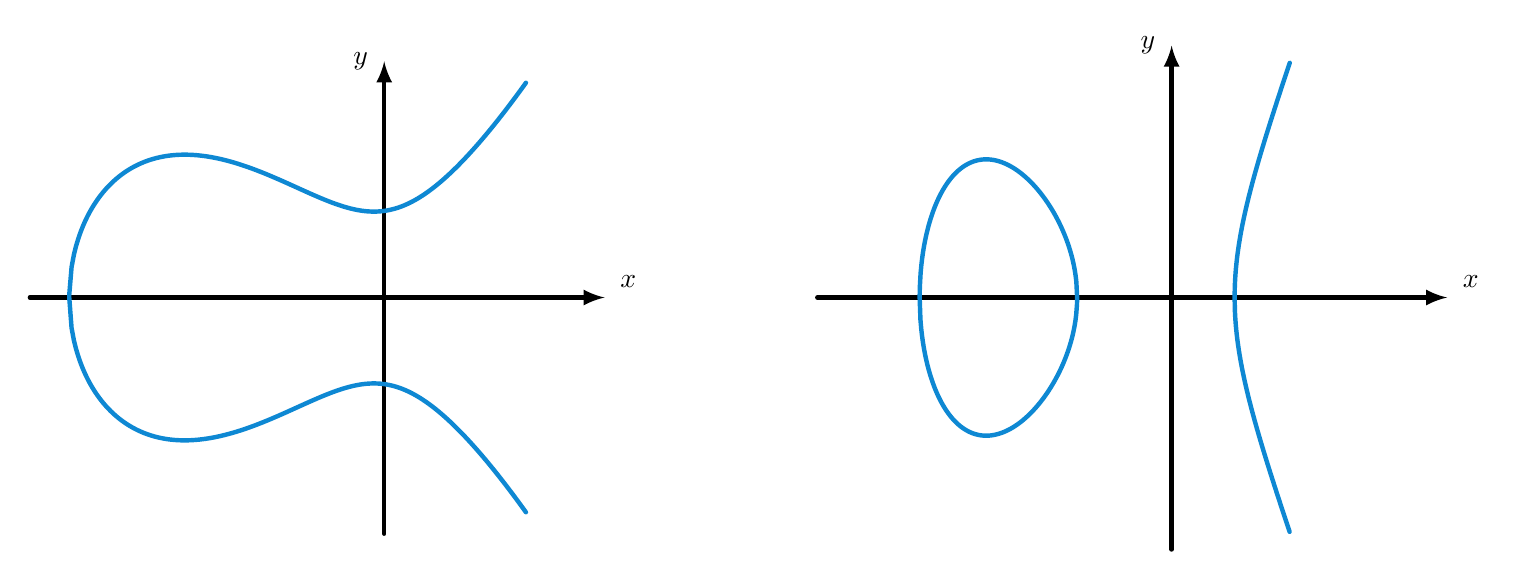
\begin{tikzpicture}[>=latex, line cap=round, line join=round]

% --- Global TikZ Styles for Consistency ---
\tikzset{
    axis/.style={
        ->,
        >=latex,
        ultra thick,
        draw=black
    },
    axisline/.style={
        ultra thick,
        draw=black
    },
    elliptic/.style={
        draw=cyan!70!blue,
        line width=1.6pt
    }
}

% =========================================================================
% --- Left Elliptic Curve: Vertically compressed ---
% =========================================================================
\begin{scope}[xshift=0cm]

    % --- Axes ---
    \draw[axisline] (-4.5,0) -- (1.8,0); % x-axis line
    \draw[axis] (1.8,0) -- (2.8,0);      % x-axis arrow

    \draw[axisline] (0,-3.0) -- (0,0);   % y-axis line
    \draw[axis] (0,0) -- (0,3.0);        % y-axis arrow

    \node at (3.1,0.2) {$x$};
    \node at (-0.3,3.0) {$y$};

    % --- Plotting with a 0.55 multiplier for a flatter look ---
    \draw[elliptic]
        plot[domain=1.80:-4, samples=200] (\x, {0.55 * sqrt(abs(\x*\x*\x + 4*\x*\x + \x + 4))})
        -- 
        plot[domain=-4:1.80, samples=200] (\x, {-0.55 * sqrt(abs(\x*\x*\x + 4*\x*\x + \x + 4))});

\end{scope}

% =========================================================================
% --- Right Elliptic Curve: Shifted left and bounded ---
% =========================================================================
\begin{scope}[xshift=10cm]

    % --- Axes ---
    \draw[axisline] (-4.5,0) -- (2.5,0); % x-axis line
    \draw[axis] (2.5,0) -- (3.5,0);      % x-axis arrow

    \draw[axisline] (0,-3.2) -- (0,0);   % y-axis line
    \draw[axis] (0,0) -- (0,3.2);        % y-axis arrow

    \node at (3.8,0.2) {$x$};
    \node at (-0.3,3.2) {$y$};

    % --- Closed Oval Component ---
    % Shifted left by 1.2 units (\x - 1.2) so it sits entirely to the left of the y-axis
    \draw[elliptic]
        plot[domain=0:-2, samples=200] (\x - 1.2, {sqrt(abs(\x*\x*\x - 4*\x))})
        -- 
        plot[domain=-2:0, samples=200] (\x - 1.2, {-sqrt(abs(\x*\x*\x - 4*\x))})
        -- cycle;

    % --- Right infinite component ---
    % Domain reduced from 3.5 to 2.7 to prevent overshooting the y-axis limits
    \draw[elliptic]
        plot[domain=2.7:2, samples=200] (\x - 1.2, {sqrt(abs(\x*\x*\x - 4*\x))})
        -- 
        plot[domain=2:2.7, samples=200] (\x - 1.2, {-sqrt(abs(\x*\x*\x - 4*\x))});

\end{scope}

\end{tikzpicture}